\documentclass[11pt]{article}

\usepackage[margin=1in]{geometry}
\usepackage{amsmath, amssymb}
\usepackage{graphicx}
\usepackage{booktabs}
\usepackage{caption}
\usepackage{hyperref}
\usepackage{float}

\title{MGT 595: Quantitative Investing \\ Problem Set 1 --- Part 1}
\author{Group: Ashley Wen, Emily Wu, Grace Gu}
\date{\today}

\begin{document}
\maketitle

\setcounter{section}{-1}

\section{Dataset Construction}

\subsection{Investment Philosophy}

\textbf{What investment philosophy guided the construction of the universe?}

This portfolio was constructed with a focus on ``Quality Growth.'' Because of
our shared interest in Information Technology and Health Care, we assigned
greater weights to these sectors for their long-term growth potential and
profitability. We also allocated a meaningful share to Energy, where structural
demand and different economic drivers could help balance the growth-oriented
holdings. Meanwhile, the portfolio maintains exposure to all 11 GICS sectors
to reduce concentration risk and avoid relying too heavily on the performance
of only a few industries.

\subsection{Candidate Pool and Screening Method}

\textbf{How were the stocks screened and selected?}

Once the number of stocks required from each sector had been determined, we
formed a candidate pool approximately twice the size of the eventual
allocation. The candidate pools included both large, established companies
and smaller firms with market capitalizations below \$5 billion.

We then compared the candidates using a simplified multifactor framework that
considered profitability, revenue growth, valuation, leverage, price momentum,
and market risk. Because the portfolio follows a ``Quality Growth'' philosophy,
greater emphasis was placed on growth and profitability. Valuation, debt,
\texttt{Beta}, and recent price movements were also considered to keep the
overall risk at a reasonable level.

\subsection{Final Stock Universe}

\textbf{Does the final universe satisfy the assignment requirements?}

The final universe contains exactly 50 U.S.-listed stocks and maintains
exposure across all 11 GICS sectors. It includes five companies with market
capitalizations below \$5 billion: \texttt{OII}, \texttt{ADUS}, \texttt{LNN},
\texttt{PLUS}, and \texttt{PLAB}. Therefore, the universe satisfies both the
sector-diversification and small-cap requirements of the assignment.

After the stocks had been selected, the 50 tickers were alphabetized before
constructing the nested portfolios used in Part 1. The first 5, 10, and 25
stocks were therefore determined by this fixed alphabetical order rather than
by their screening rankings. This makes the comparison across portfolio sizes
more neutral by preventing us from intentionally placing our most preferred
stocks in the smaller portfolios.

\subsection{Data Collection}

\textbf{How were the historical prices obtained?}

Adjusted monthly closing prices for all 50 stocks and the S\&P 500
(\texttt{\^{}GSPC}) were downloaded using \texttt{yfinance} with
\texttt{interval="1mo"} and \texttt{auto\_adjust=True}. The final sample covers
January 2010 through the most recent complete month and contains 200 monthly
return observations.

\subsection{Missing-Data Validation}

\textbf{Were any stocks or months removed because of missing data?}

All 50 stocks had complete monthly coverage over the common sample period.
Therefore, no ticker exceeded the assignment's 5\% missing-data threshold, no
ticker was dropped or replaced, and no month was removed during complete-case
alignment.

\subsection{Extreme-Return Validation}

\textbf{Were potentially unusual monthly returns investigated?}

As part of the data-validation process, monthly returns below $-50\%$ or above
$+200\%$ were flagged for investigation rather than automatically removed.
Three observations met this criterion: \texttt{EXEL} returned approximately
$-63.0\%$ in September 2014, while \texttt{OII} and \texttt{OKE} each declined
by approximately $70\%$ in March 2020.

The latter two observations coincided with the COVID-19 market disruption and
the collapse in oil prices. Because the flagged observations appeared to
represent genuine market movements rather than data errors, they were retained
in the final dataset.

\subsection{Bias Acknowledgement}

\textbf{How should selection and survivorship bias affect the interpretation
of the results?}

Our sample is subject to both selection and survivorship bias. The selection
process intentionally favored companies with stronger current fundamentals,
particularly in Information Technology and Health Care. As a result, the
portfolio's returns, volatility, and covariance structure may not be
representative of the broader U.S. stock market.

In addition, requiring continuous historical data back to January 2010
restricted the sample to companies that are still listed today. Firms that
failed, were delisted, or were acquired before the selection date were excluded
by construction. Therefore, average returns may appear higher and downside risk
may appear lower than they would in a universe that included unsuccessful
firms, although this effect is not guaranteed for every excluded company.

The diversification patterns reported in Part 1 should consequently be
interpreted as evidence for this particular group of selected surviving firms,
rather than as general estimates for all stocks that were investable in January
2010. Alphabetizing the tickers makes the comparison among the nested
portfolios more neutral, but it does not eliminate the selection bias in the
original 50-stock universe.

\subsection{Dataset Summary}

\begin{itemize}
    \item \textbf{Investment philosophy:} Quality Growth
    \item \textbf{Number of stocks:} 50
    \item \textbf{GICS sectors represented:} 11
    \item \textbf{Stocks below \$5 billion:} 5
    \item \textbf{Market benchmark:} S\&P 500 (\texttt{\^{}GSPC})
    \item \textbf{Return frequency:} Monthly
    \item \textbf{Final number of monthly returns:} 200
    \item \textbf{Stocks dropped or replaced:} None
    \item \textbf{Months removed during alignment:} None
    \item \textbf{Extreme observations flagged and retained:} 3
\end{itemize}

\section*{Question 1(a): Diversification and Basic Statistics}

We form equal-weight portfolios using the first 5, 10, 25, and all 50
tickers in fixed alphabetical order. For each portfolio, the sample mean and
sample standard deviation of monthly returns were computed.

\begin{table}[H]
\centering
\caption{Equal-weight portfolio statistics}
\begin{tabular}{cccc}
\toprule
$N$ & Sample Mean & Sample Std.\ Dev. \\
\midrule
5  & 1.6362\% & 4.9518\% \\
10 & 1.6393\% & 4.4471\% \\
25 & 1.5201\% & 4.5803\% \\
50 & 1.5960\% & 4.4970\% \\
\bottomrule
\end{tabular}
\end{table}

\begin{figure}[H]
\centering
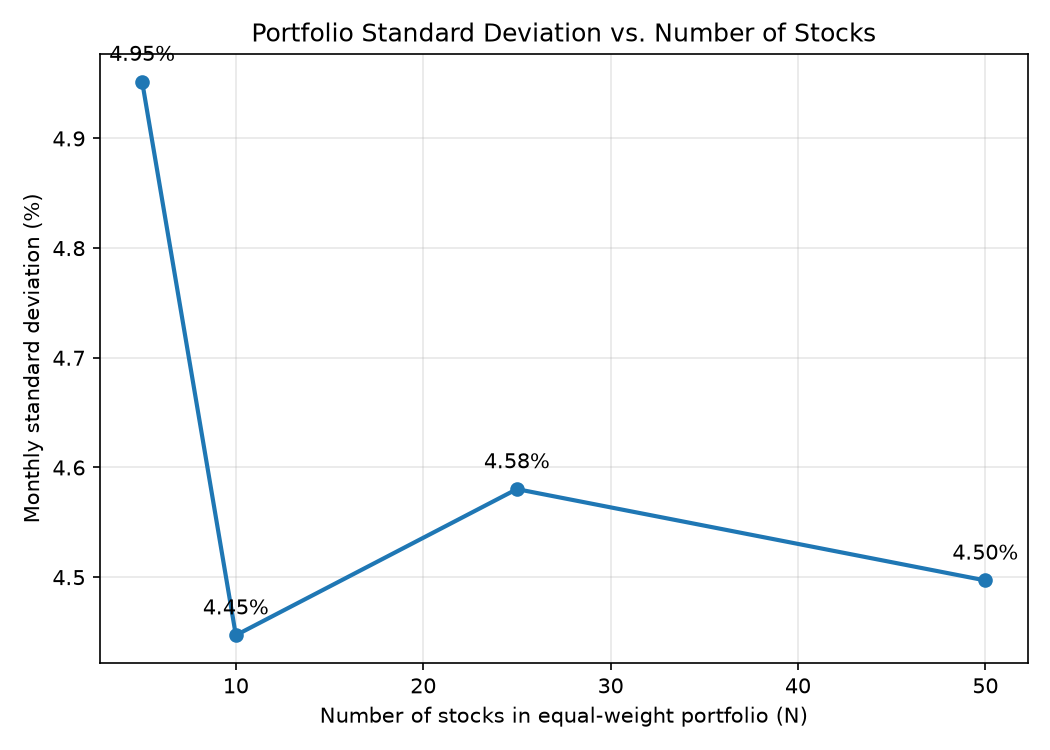
\includegraphics[width=0.75\textwidth]{1a_diversification_curve.png}
\caption{Portfolio standard deviation vs.\ number of stocks ($N$)}
\end{figure}

\paragraph{Discussion.} Although the curve is not perfectly monotonic, it shows an overall downward and flattening pattern. This is broadly consistent with diversification theory: adding stocks generally reduces firm-specific risk, but a realized nested sample does not guarantee that volatility falls with every addition.

Despite the decline, the standard deviation would not reach zero even if the porfolio grows larger. As the portfolio becomes larger, firm-specific risk declines, butcommon covariance and systematic market risk remain and cannot be diversified
away.

\section*{Question 1(b): Variance Decomposition}

For each equal-weight portfolio, we decomposed total variance into a
contribution from individual stock variances and a contribution from
covariances, using
\[
\mathrm{Var}(r_p) = \frac{1}{N}\,\overline{\mathrm{Var}} +
\frac{N-1}{N}\,\overline{\mathrm{Cov}},
\]
where $\overline{\mathrm{Cov}}$ is backed out algebraically from the
portfolio variance and the average individual variance, without directly
estimating the full pairwise covariance matrix.

\begin{table}[H]
\centering
\caption{Variance decomposition by portfolio size}
\begin{tabular}{ccccccc}
\toprule
$N$ & Avg.\ Var. & Avg.\ Cov. & Port.\ Var. & Var.\ Contrib. & Cov.\ Contrib. & \% from Var. \\
\midrule
5  & 0.007284 & 0.001244 & 0.002452 & 0.001457 & 0.000995 & 59.41\% \\
10 & 0.006481 & 0.001477 & 0.001978 & 0.000648 & 0.001330 & 32.77\% \\
25 & 0.007113 & 0.001889 & 0.002098 & 0.000285 & 0.001813 & 13.56\% \\
50 & 0.007485 & 0.001911 & 0.002022 & 0.000150 & 0.001873 & 7.40\% \\
\bottomrule
\end{tabular}
\end{table}

\begin{figure}[H]
\centering
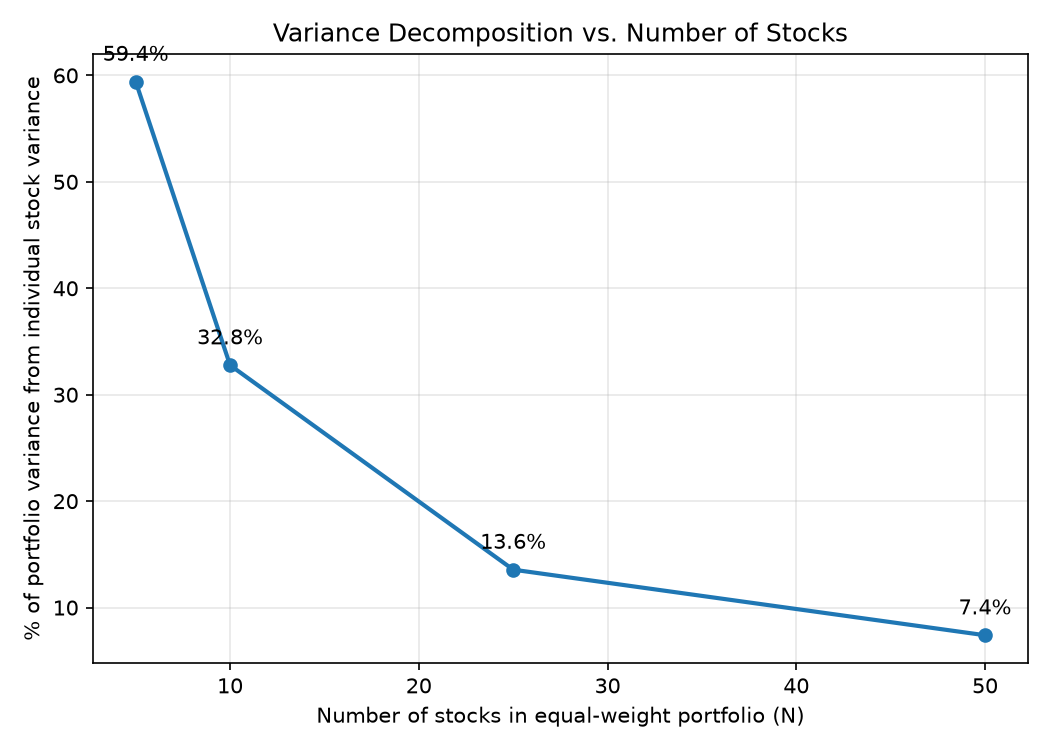
\includegraphics[width=0.75\textwidth]{1b_variance_decomposition.png}
\caption{Percentage of portfolio variance from individual stock variance vs.\ $N$}
\end{figure}

\paragraph{Discussion.} Compared with Question 1(a), this curve shows a much
smoother decline. As the number of stocks increases, the percentage of
portfolio variance attributable to individual stock variances decreases,
making the covariance contribution increasingly important.

This is consistent with diversification theory. Because the
individual-variance component is divided by $N^2$, it is gradually diluted as
the portfolio grows and may approach zero. However, total portfolio variance
does not approach zero because covariance persists as stocks remain exposed to
shared market and economic conditions.


\end{document}
